\chapter{The TTA16 and RISC16 Processor Cores}
\label{CPU}

OpenVGA is designed to use a processor logic core for initialisation, mode
setting, and data processing tasks. Two processors were developed for these
tasks, the first was TTA16, a novel, 16-bit, transport-triggered processor. The
second processor that was developed, RISC16, a 16-bit, RISC processor
architecture, was for comparison with TTA16, and for its relative ease of
programming in assembly language.


\section{Processor Architectures}
An aim for OpenVGA's processor was to be fast enough to emulate VGA text-mode.
After evaluating existing FPGA-based, processor logic cores (see
Table~\ref{SUMMARY_CPU_Table}), it was decided to develop a new processor to meet
this speed and size criteria. Popular Instruction Set
Architectures
(\gls{isa}s) were considered for the OpenVGA processor. These included Complex
Instruction Set Computer (\gls{cisc}), RISC, and Very Long Instruction Word (\gls{vliw}) architectures.

Figure~\ref{CPU_Sched} gives a breakdown of the tasks that a compiler and
processor must perform, and the division of these tasks for differing processor
architectures. Modern superscalar CISC and RISC processors use a lot of die area
for functionality other than transporting and processing data. This often
includes hardware for instruction decoding, out-of-order execution, speculative
execution, and branch prediction~\cite{parhami2005cam}. TTA processors typically
do not have these features~\cite{corporaal:tta}, with most of the logic gates
used for data transports and Functional Units (\gls{fu}s), resulting in smaller processor designs.

\begin{figure}[h!]
\begin{center}
\includegraphics[width=\linewidth]{images/hardware_sched.pdf}
\caption[The division of responsibilities between hardware and compiler]{The
division of responsibilities between hardware and compiler. (Image
from~\cite{corporaal1999tmi})}
\label{CPU_Sched}
\end{center}
\end{figure}

An efficient architecture would operate at a high frequency, have a high FU
utilisation rate, and use minimal logic resources. FPGAs have reduced frequency
and fewer logic gates than similar generation ASICs so a smaller, faster
processor architecture is arguably even more important. This is why a TTA
processor was chosen for OpenVGA. But the complexity of generating efficient
firmware code for TTA16 is why a second processor, RISC16, was developed.

TTA processors were investigated (designed, built, programmed, and characterised)
at the Technical University of Delft by Henk Corporaal et.
al.~\cite{corporaal1999tmi, corporaal:tta, corporaal1993maa} during the 1990s.
Additional TTA research has focused on the automatic generation of the HDL
source-code for TTA processor logic cores~\cite{hoogerbrugge1995ast,
jaaskelainen2007cta}. The goal has been to develop application-specific
processors for certain tasks, like image processing
applications~\cite{corporaal1999tmi}.

Xilinx Spartan-3 FPGA logic resources, and their latencies, also affect the
choice of processor architecture, and which features can be implemented
efficiently as well. The Spartan-3 has 18-bit embedded multipliers, fast
carry-chain logic, 16-entry and 2~kB RAM primitives, DCMs (Digital Clock
Modules), and some additional multiplexing primitives\footnote{The high
combinatorial logic delays of multiplexers synthesised for Spartan-3 FPGAs
influenced many design decisions. Even with some hardware support for wide
multiplexers these were still quite slow~\cite{Xilinx_SP3_DS}.}. These available
FPGA resources influenced the architectures evaluated, and the design choices
made.

Both of the processor logic cores developed for OpenVGA, TTA16 and RISC16,
feature a data word-size of 16-bits for two main reasons:
\begin{itemize}
  \item Functional units are typically half the size of those for 32-bit
  processors so the resulting processor will be a lot smaller.
  \item Wider signal paths use more routing resources, and are more difficult
  for the Xilinx PAR tool to route, usually resulting in lower frequencies.
\end{itemize}


\section{Shift Registers as Program Counters}
Rather than use a standard, base-2 incrementer for each processor's Program
Counter (\gls{pc}), a Multiple
Feedback Shift Register (\gls{mfsr})~\cite{MFSR_List} is used as the PC incrementer for both
TTA16 and RISC16. The count order of an MFSR is very different to standard base-2
incrementers. To illustrate this different increment sequence, an application of
MFSRs is for use as pseudo-random sequence generators. For a maximal-cycle MFSR
having $n$-bits, the cycle length is $2^n-1$, and can be implemented with a
maximum of just one layer of logic gates (see Figure~\ref{CPU_MFSR8}).

The reason for using MFSRs as PCs is due to the extremely small combinatorial
logic delay, just the propagation delay through one FPGA Look-Up
Table (\gls{lut}) and some routing
fabric. This allows the PC increment and branch logic to have very low latency,
avoiding the requirement pipeline registers, or becoming the processor's critical
path and limiting maximum frequency.

\begin{figure}[h!]
\begin{center}
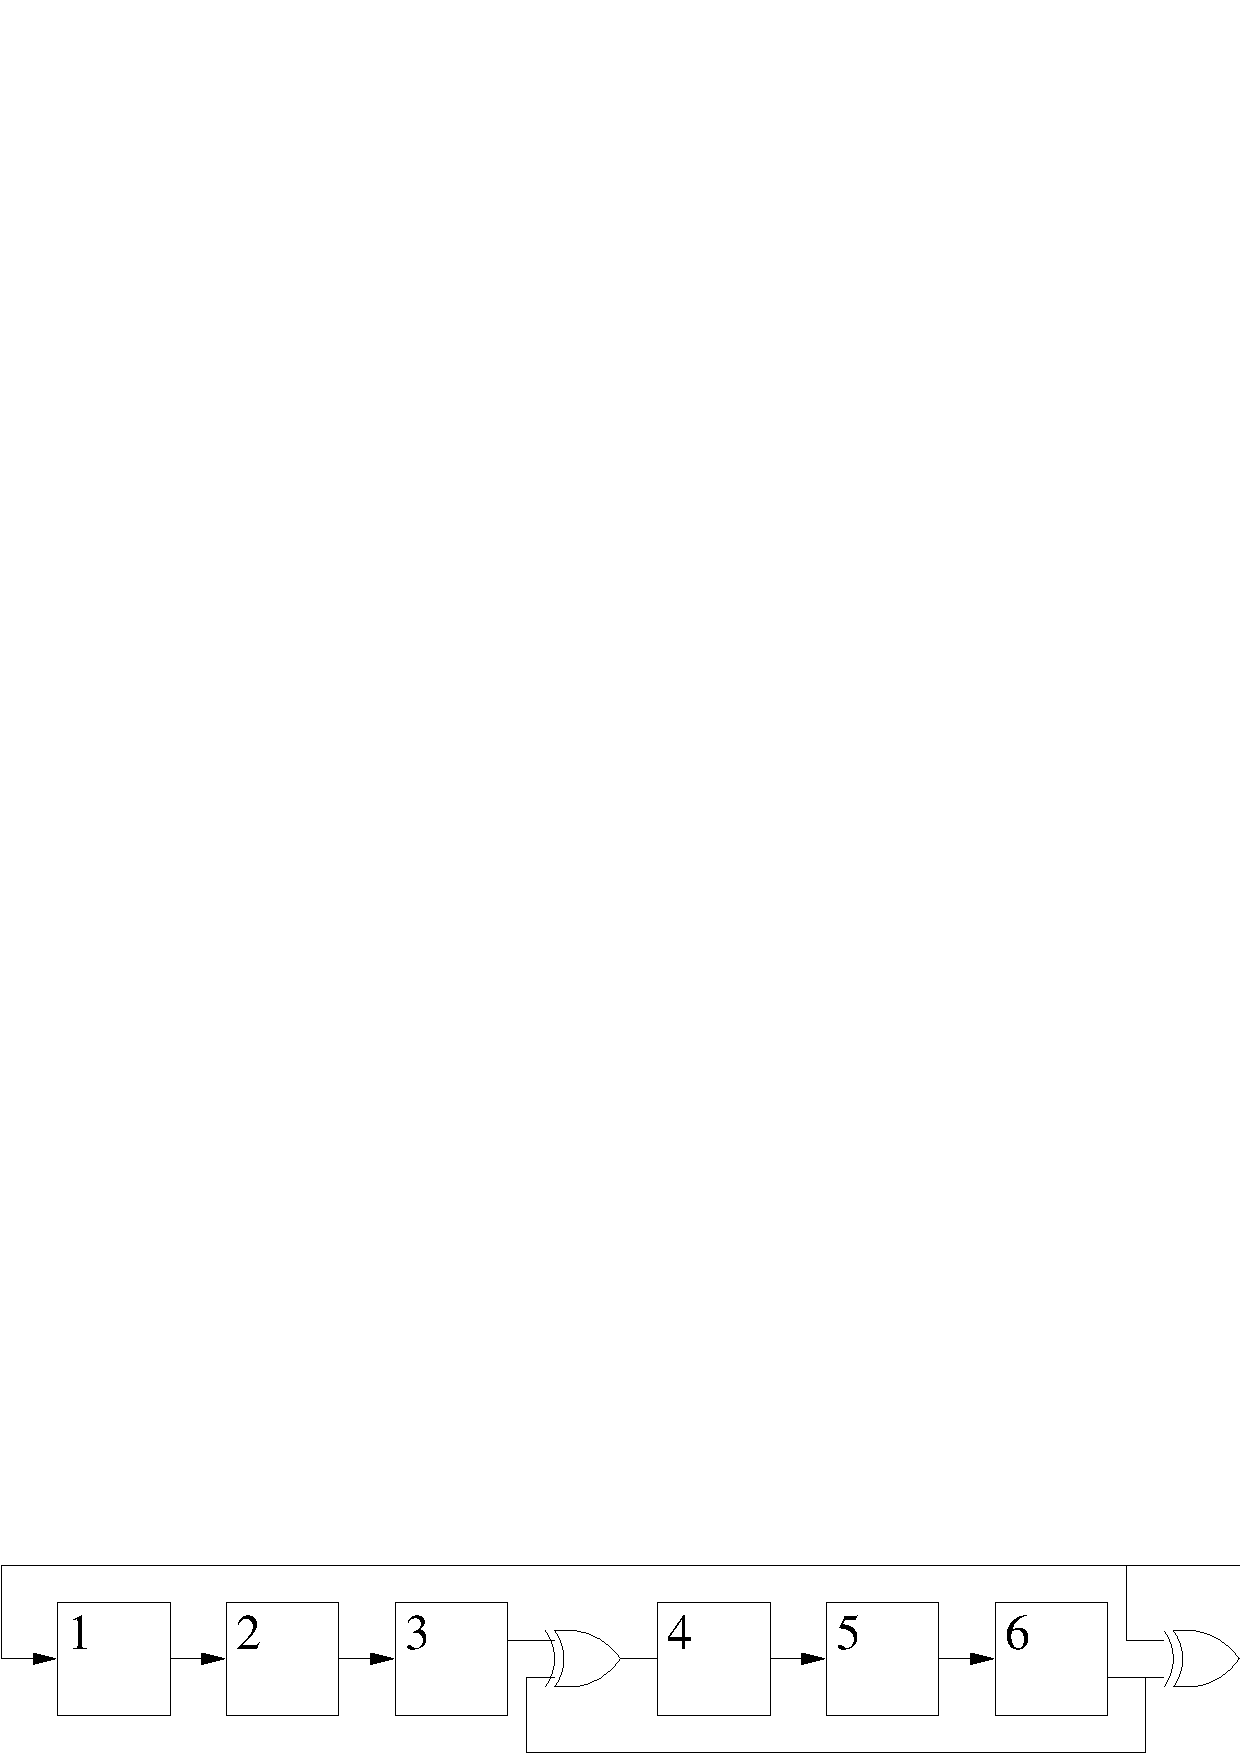
\includegraphics[width=\linewidth]{images/mfsr8.pdf}
\caption[An 8-bit MFSR with a cycle size of 255]{An 8-bit MFSR (Multiple
Feedback Shift Register) with a cycle size of 255. The total logic required is
only eight D-type flip-flops and two XOR logic gates. \textit{Image courtesy
of R. Ward}~\cite{MFSR_List}}
\label{CPU_MFSR8}
\end{center}
\end{figure}


\section{Processor Performance}
To improve the performance of a processor, the biggest gains are made by making
the common operations fast~\cite{Comp_Arch}. The primary computational task of
OpenVGA's processor is to convert data sent to OpenVGA into the framebuffer's
data format. This consists of mainly arithmetic, bit-wise logic, and memory
operations. Arithmetic and logical operations take just one clock cycle. Memory
operations are far slower but a fast data-cache has been developed (see
Section~\ref{MEM_Cache}), reducing the average delay to only about five processor
clock cycles.


% \subsection{Amdahl's Law}
Amdahl's law defines the speedup obtained from a given enhancement made to a
machine~\cite{Comp_Arch}. This speedup is based on the performance for the entire
task, with and without the enhancement, $\tau_E$ and $\tau_O$ respectively. For a
given enhancement to a CPU, the speedup is the ratio defined as

\[
\mathrm{Speedup} = \frac{\tau_O}{\tau_E}
\]

Amdahl's Law allows the effect of enhancements to the CPU to be objectively
evaluated. For example, consider the question: ``How much of a performance effect
does doubling the number of processor data-transports and FUs give?''

\begin{flushleft}\textbf{Answer:} A memory operation for the text-mode conversion
algorithm typically takes about 5 clock cycles, due to the benefit of
data-caching. If about one third of the instructions contain memory operations
(see Section~\ref{CACHE_Justification}), and all other operations complete in one
clock cycle, and about two million memory accesses are required to redraw one
frame, then the time in cycles to redraw one frame is

\begin{eqnarray*}
\tau_O	& = & 5 \times 2\times10^6 + 4\times10^6 \\
		& = & 14\times10^6
\end{eqnarray*}

If the number of transports and functional units are doubled, giving a perfect
speedup of two for non-memory instructions, then the total speedup would be

\begin{eqnarray*}
\mathrm{Speedup}	& = & \frac{\tau_O}{\tau_E}	\\
					& = & \frac{14\times10^6}{12\times10^6}	\\
					& \approx & 1.17	\\
\end{eqnarray*}
\end{flushleft}

The resulting CPU would nearly be twice as large though. The actual speed-up
factor will be less than two because of scheduling difficulties. And the Xilinx
PAR tool would find the design harder to route, likely reducing processor
operating frequency too. So doubling the number of transports would not be an
efficient modification in this case since the FPGA logic resources are limited
and the speedup minimal.


\section{Tools \& Testing}
One of the processors designed and implemented within OpenVGA, TTA16, has an
unsual architecture, and it would be a non-trivial task to adapt an existing open
source assembler, and especially a compiler, to this architecture. It would have
been extremely tedious to generate large quantities of object code too. Therefore
an assembler was needed for both TTA16 and RISC16.

Testing the two processors was initially done with the Icarus Verilog simulator,
and later with hardware testbenches. Simple TTA16 and RISC16 programs were
written for processor testing to verify correct operation of the FUs. The CPU of
the host PC can access all of OpenVGA's memory using a Linux kernel module.

\subsection{Object Code Generation}
Processors execute instructions in the form of object code, which is a binary
representation of an instruction. Typically, assemblers, interpreters, and
compilers are used to generate object code. There are currently no interpreters
or compilers that have TTA16 or RISC16 as an output target since these processors
have custom instruction sets. There is an assembler for each of these processors
though.

\subsubsection{TTA16 Assembler}
\filedescript{Roy Ward, Patrick Suggate}{assemble}{A general-purpose TTA
assembler which loads an XML processor description from a
file prior to assembly.}{/data/tta16.xml}{/src/fw\_tta16/*.S}{GPL}

An assembler was created by R. Ward~\cite{XML_Assembler} for another project, and
additional features were added by him to assist this project. This assembler
reads in a processor definition file, which is stored as an XML file, and then
assembles the assembly language source file in accordance to the definition in
the XML file. This assembler was designed for TTA applications and it supports
explicit Instruction Level Parallelism (\gls{ilp}) (see the TTA16 programming
guide in Appendix~\ref{TTAPROG_TTA16_memcpy} for an example of this).

Below is an excerpt from \texttt{tta16.xml}, the file defining the TTA16
instruction set. This fragment encodes the available destination registers for
transport-0 of TTA16\footnote{This bit-field is called $DST0$ in the instruction
format diagram, see Figure~\ref{TTA_Instruction_Format}} , and has been included
to demonstrate the syntax. The XML encoding is very general purpose, and has been
used for other TTA processors as well~\cite{TTA_Ray_Trace}.

\begin{center}
\begin{minipage}{0.8\linewidth}
\footnotesize
\verbatiminput{source/tta16_excerpt.tex}
\normalsize
\end{minipage}
\end{center}

\noindent The first line in a TTA16 assembly source file is typically:
\begin{center}
\begin{minipage}{0.5\linewidth}
\begin{verbatim}
architecture:tta16
\end{verbatim}
\end{minipage}
\end{center}

This line specifies the name of XML file to use when assembling this file and
this line has to precede any assembly language. Comments may precede this line,
and since the \texttt{m4} macro processor was used as a preprocessor with this
assembler, to allow the use of constants and macros for common tasks, macro
definitions will often be at the start of TTA16 assembly files too.

A TTA16 instruction encodes the move operations for each of its four transports.
Each of these four \texttt{move} fields are separated by commas, and an empty
field indicates no-operation for that transport within the current instruction.

Arrows (a minus and a greater-than, \texttt{->}) are a required part of the
assembly syntax and they graphically indicate the direction of data flow. Curly
braces surround all instructions, and instructions can be preceded by an optional
label, before the braces. More information on TTA16 assembly and programming is
in Appendix~\ref{TTA_Programming}, but here is an example of the TTA16 assembly
syntax:
% \footnotesize
\begin{center}
\begin{tabular}{l l l l l l l l l}
\tt loop: & \tt \{r1 & \tt ->rad, & \tt 2 & \tt ->sub, & & & \tt ,r2 \tt
\}
\end{tabular}
\end{center}
Shown above is a label, \texttt{loop:}, two general-purpose registers
(\texttt{r1} and \texttt{r2}), and two special-purpose registers
(\texttt{rad} and \texttt{sub}). The third \texttt{move} field is empty,
indicating no-operation, and the fourth transport has only one argument,
\texttt{r2}. This is the source for the data-move, the destination is always the
common ALU operand register \texttt{com}, and is therefore excluded from the
syntax.


\subsubsection{RISC16 Assembler}

\filedescript{Patrick Suggate}{r16asm.py}{A simple RISC16
assembler.}{/src/r16asm.py, /src/CodeCleaner.py, /src/AsmParse.py,
/src/Emit.py}{/src/fw\_risc16/*.S}{GPL}

RISC16 uses a custom assembler, written in Python specifically for this
processor. Example code written for this assembler is shown in
Appendix~\ref{RISCPROG_Memcpy}. RISC architectures are not explicit-ILP
processors, and the syntax used with the TTA assembler is somewhat cumbersome for
RISC16. Additionally, RISC16 had some instructions that were hard to define
within the XML processor definition file (especially the immediate constant field
of the \texttt{i12} instruction prefix). This justified the creation of yet
another assembler.

\noindent The general form of a valid line of assembly code that is accepted by
this assembler is:

\begin{center}
\tt		[label:] mnemonic [arguments]
\end{center}

The \texttt{label:} field is used to label the destination of branches, and to
label constants so they can be referenced within the code. The \texttt{mnemonic}
field is a keyword identifying the desired instruction, which is translated into
an \gls{opcode} (condensed form of operation-code) in the final phase of the
assembler. Fields surrounded by square braces indicate that the field can be
optional. All constants are required to have a label, and most instruction
require arguments.

An overview of the algorithm the assembler uses to generate an output file is:

\begin{enumerate}
  \item Parse command-line options for the input file name, the optional output
  file name, and the assembler options.
  \item Read in assembly file, line-by-line. Line numbers are
  stored, with each line, at this point. This is needed so useful error
  messages can be generated later.
  \item Remove comments and extra white-spaces, throwing away lines containing
  no code or no assembler directives.
  \item Tokenise each of the remaining lines according to the simple format
  discussed above.
  \item The parser takes the stream of tokens, builds a table of constants, and
  then a table of branch destination labels. The next parse step is
  evaluating the instruction arguments, which involves substituting any
  labels, in the arguments, for its corresponding constant or address value.
  The final parse step is to evaluate any argument that represents a numerical
  value, the set arithmetic and bit-wise logical operations used in the C
  language is accepted.
  \item Since both TTA16 and RISC16 use an MFSR instead of a standard PC
  incrementer, the generated object code needs to be reordered according to
  the MFSR count order. Since the count order is pseudo-random, it will span
  the entire instruction RAM block(s), so before reordering the instruction
  stream, it is padded with \texttt{nop} (no-operation) instructions so that it
  contains the same number of instructions as the block RAMs can hold.
  \item The parsed and reordered instruction mnemonics and arguments are
  matched against valid instruction formats, and upon match, the hexadecimal
  representations of the object code is then emitted to the output file.
\end{enumerate}


\subsection{Processor Testing and Testbenches}
Initially, each FU was developed and tested using the FOSS (Free and Open-Source
Software) simulator Icarus Verilog\footnote{Icarus Verilog is available on the
Internet from http://www.icarus.com/eda/verilog/}. Processors can be very
difficult to debug, especially RISC16 with its many hazard detection flags and
states, so it was important that the components were well tested first. Another
FOSS Electronic Design Automation (\gls{eda}) application, GtkWave\footnote{GtkWave is available on
the Internet from http://gtkwave.sourceforge.net/} was used to display the timing
diagrams of the simulated signals, which were saved to a \gls{vcd} (Value Change Dump) output file by Icarus.

When a processor had been developed to the point where it simulated as expected,
larger quantities of test code were written, with a disassembler coded within
the processors HDL source displaying the instructions (with input and output
values) being executed. The MMIO functionality and correct data cache operation
could then be verified.

Once a design was believed to operate correctly, hardware testbenches were
synthesised and uploaded to OpenVGA, at first just running code for a trivial
task like flashing some LEDs. Figure~\ref{TTA16_Synthesis} shows the synthesiser
output for one of the TTA16 hardware testbenches. As can be seen, TTA16 is very
fast for a processor implemented on Spartan-3\footnote{It is often estimated that
an FPGA has about one-tenth the performance of an ASIC made with the same
manufacturing process, in this case 90 nm.}.

The Verilog synthesiser used was ISE WebPack$^{TM}$ 9.1 developed by Xilinx,
since it is free of charge, though proprietary, and available for both the Windows and
GNU/Linux operating systems. Being free, it keeps with the goal of OpenVGA being
a low-cost platform for development.


\begin{figure}[h!]
\begin{center}
\Ovalbox{%
	\begin{minipage}{0.9\linewidth}
		\begin{center}
		\begin{minipage}{0.8\linewidth}
\begin{verbatim}

Timing summary:
---------------

Timing errors: 0  Score: 0

Constraints cover 2115 paths, 0 nets, and 1452 connections

Design statistics:
   Minimum period:   5.249ns (Maximum frequency: 190.512MHz)
   Minimum input required time before clock:   6.874ns
   Maximum output delay after clock:   9.816ns


Analysis completed Wed Dec 24 08:08:07 2008
-------------------------------------------
\end{verbatim}
		\end{minipage}
		\end{center}
	\end{minipage}}
\caption[TTA16 synthesis timing report]{Xilinx Place and Route (PAR) report
showing the synthesised TTA16 hardware testbench timing and routing information.}
\label{TTA16_Synthesis}
\end{center}
\end{figure}





%%%%%%%%%%%%%%%%%%%%%%%%%%%%%%%%%%%%%%%%%%%%%%%%%%%%%%%%%%%%%%%%%%%%%%%%%%%%%
%%%%%%%%%%%%%%%%%%%%%%%%%%%%%%%%%%%%%%%%%%%%%%%%%%%%%%%%%%%%%%%%%%%%%%%%%%%%%
\section{TTA16}
\label{TTA16}

\mmodule{Patrick Suggate}{tta16}
{A 16-bit, TTA processor logic core designed for use with FPGAs.}
{/rtl/cpu/tta16/tta16.v, /rtl/cpu/tta16/tta16.xml,
/rtl/cpu/tta16/tta\_stream4to4.v, /rtl/cpu/tta16/tta\_stream4to8.v,
/rtl/cpu/tta16/tta\_stream8to8.v, /rtl/cpu/fastbits.v}
{/sim/cpu/tta16\_tb.v}{GPL}

TTA16, is a small, fast, 16-bit, transport-triggered, processor logic core
designed for OpenVGA initialisation, state management, and the data processing
tasks for emulating VGA functionality. TTA16 features a three-stage pipeline,
four data transports, explicit ILP, 16 general purpose registers, up to 32-bit
memory address support, logic and arithmetic operations, a multiplier, a fast
local instruction store, and a fast Wishbone bus interface to access OpenVGA
Wishbone bus peripherals, including the system memory.

TTA16 is a partially-connected TTA, each FU can only get data from, and place
data on, a subset of the processor transports. The FU and data-transport
connectivity of TTA16 is shown in Figure~\ref{TTA16_Tranport_View}. Partially
connected TTAs allow the use of smaller multiplexers for connecting FUs to
transports, resulting in smaller and faster designs~\cite{arnold1997dtr}.

\begin{figure}[h!]
\begin{center}
\includegraphics[width=\linewidth]{diagrams/tta16_henk.pdf}
\caption[TTA16 transports and functional units overview]{TTA16 transport-based
diagram which shows the connections between transports and FUs.}
\end{center}
\label{TTA16_Tranport_View}
\end{figure}

Even though TTA16 is a very capable processor, when synthesised for the Spartan-3
architecture TTA16 uses only approximately 220 logic slices\footnote{This is when
XST is set to optimise for speed, when optimising for size it uses even less.}
which is very small for the feature set. Additionally, the maximum clock rate at
which it will run is up to 190 MHz (see Figure~\ref{TTA16_Synthesis}), very fast
for a processor implemented within the Spartan-3 FPGA family. A comparison with
other Spartan-3 based processors is shown in Table~\ref{SUMMARY_CPU_Table}.


\subsection{Introduction to TTA Processors}
A TTA processor is different from more common processors, like RISC and CISC
based processors such as ARM, SPARC, x86, Power, and MIPS. TTA instructions are
simply a list of data moves for each transport that the processor has to perform.
For comparison, instructions of more traditional architectures typically specify
the desired operation and the data to use for that operation.

To perform useful work, processors need FUs (Functional Units) that carry out
some operation, like branching, memory load and store, and subtraction and other
calculations. Work is performed within a TTA processor by transporting values to
special purpose registers, some of which can trigger side-effects, like
computations. There are three main classes of registers

\begin{itemize}
  \item Trigger Registers: These trigger the start of operations within FUs.
  The operations which are initiated depend on the FU, they can be an
  operation like a memory write, or a subtract, or whatever computations the FU
  supports.
  \item Operand Registers: These supply additional values for an operation, a
  subtract requires both a subtrahend and a minuend, for example. Unlike
  trigger registers, writing to an operand register has no side-effects. The
  number of operand registers required by a FU varies, and can even be zero.
  \item Result Registers: These are the results of computations by FUs, they
  can have a latency of zero or more cycles, and FUs can have more than one
  result register, like the multiplier (see Section~\ref{TTA_Multiply}) for
  example.
\end{itemize}

Figure~\ref{TTA_Simple_Add} demonstrates how to perform a calculation in a TTA
processor, in this case an addition. RISC-type assembly code is given for
comparison. The simple addition example looks to be a clear win to the RISC
processor, even if it is assumed that a TTA can be made to operate at a 50\%
higher clock rate (see Table~\ref{SUMMARY_CPU_Table}).

Also note that the RISC instruction reads two values from the Register
File (\gls{rf}, \texttt{r0} and
\texttt{r1}), and writes back one (\texttt{r0}) This requires the RF to have a
bandwidth of three operations per clock cycle, or else it will take longer than a
single cycle to complete, or maybe affect/restrict other instructions.

\begin{table}[h!]
\begin{center}
\Ovalbox{
	\begin{tabular}{l l}
	\begin{minipage}{0.4\linewidth}
    	\begin{center}
		\begin{tabular}{l l}
        	\multicolumn{2}{c}{RISC-type instructions}	\\
        	\\
	    	\texttt{add} & \texttt{r0, r0, r1}	\\
	    		&				\\
	    		&				\\
	    \end{tabular}
        \end{center}
	\end{minipage} &
	\begin{minipage}{0.4\linewidth}
    	\begin{center}
		\begin{tabular}{l l l l}
        	\multicolumn{4}{c}{TTA-type instructions}	\\
        	\\
			\tt	\{\tt r0 & \tt -> & \tt add & \} \\
			\tt	\{\tt r1 & \tt -> & \tt add$_t$ & \}\\
			\tt	\{\tt sum & \tt -> & \tt r0 & \} \\
    	\end{tabular}
        \end{center}
	\end{minipage}	\\
\\
	\end{tabular}
}
\caption[A simple addition operation to demonstrate the TTA concept]{A simple
addition operation to demonstrate the TTA concept. The addition is only
initiated once a write is made to the addition-trigger register (add$_t$).}
\label{TTA_Simple_Add}
\end{center}
\end{table}


For the second example, lets say the task is to sum four numbers, stored in
\texttt{r0-3}, and the example TTA now has an ILP of two\footnote{An ILP of
four~\cite{corporaal1993maa} is common but much higher than this was experimented
with by Henk Corporaal\cite{corporaal1993maa}}. As Figure~\ref{TTA_Accumulate}
shows, the new TTA code now fares a little better, it can even be considered to
win if it can operate at a 50\% percent higher clock rate. The TTA still requires
less register-file bandwidth as well, five accesses compared to nine of the RISC.

\begin{table}[h!]
\begin{center}
\Ovalbox{
	\begin{tabular}{l l}
	\begin{minipage}{0.4\linewidth}
    	\begin{center}
		\begin{tabular}{l l}
        	\multicolumn{2}{c}{RISC-type instructions}	\\
        	\\
	    	\texttt{add} & \texttt{r0, r0, r1}	\\
	    	\texttt{add} & \texttt{r0, r0, r2}	\\
	    	\texttt{add} & \texttt{r0, r0, r3}	\\
	    		&				\\
	    \end{tabular}
    	\end{center}
	\end{minipage} &
	\begin{minipage}{0.5\linewidth}
	\begin{tabular}{l l l l l l l}
        	\multicolumn{7}{c}{TTA-type instructions}	\\
        	\\
	\tt	\{\tt r0 & \tt -> & \tt add, & \tt r1 & \tt -> & \tt add$_t$ & \} \\
	\tt	\{\tt r2 & \tt -> & \tt add, & \tt sum & \tt -> & \tt add$_t$ & \}\\
	\tt	\{\tt r3 & \tt -> & \tt add, & \tt sum & \tt -> & \tt add$_t$ &	\}\\
	\tt	\{		 &		  &			 & \tt sum & \tt -> & \tt r0 & \} \\
    \end{tabular}
	\end{minipage}	\\
\\
	\end{tabular}
}
\end{center}
\caption[TTA Accumulate Example]{TTA Accumulate Example. Accumulate four
numbers and store the result in \texttt{r0}. This TTA has an ILP of
two, meaning two data moves are performed every clock cycle.}
\label{TTA_Accumulate}
\end{table}

Due to TTA16's explicit ILP, four data moves occur per instruction. TTA16 is not
fully connected though, each execution stream cannot access all of the processors
registers, just a smaller subset. This approach makes the transports simpler, and
therefore faster, and if the connections are chosen well, the net effect is a
performance increase~\cite{arnold1997dtr} due to allowing a higher clock rate.

Even with four moves per clock, TTA16 still required less RF bandwidth than
RISC16 (a general feature of TTAs~\cite{hoogerbrugge1994rfp}), so the RF is only
half the size of RISC16 (see Section~\ref{RISC16_RF}), 16 Spartan-3 slices (32
LUTs) versus 32 of RISC16. Within OpenVGA, the total RF bandwidth of TTA16 is
identical to RISC16 since a two port RF operating at 150~MHz has the same
bandwidth as three ports at the 100~MHz of RISC16\footnote{The operating
frequencies of TTA16 and RISC16 are lower than their absolute maximum values due
to routing factors, the data cache frequency, and the Wishbone bus clocks.}.


\subsection{Internal Tri-States vs. Multiplexers}
Multiple FUs are connected to the four transports of TTA16, but since only one FU
result register can place its value onto a transport during any given clock
cycle, there needs to be hardware that selects the register to be placed on the
transport. Typically, multiplexers and internal tri-states are used, but the
Spartan-3 family does not include internal tri-states, unlike previous FPGA
families from Xilinx~\cite{Xilinx_SP3_DS}\footnote{Internal tri-states were
implemented within the Virtex II Family via primitives called TBUFs. This was
often of limited value since the number was relatively scarce and the locations
fixed. The Spartan-3 does not have any TBUFs.}.

The Spartan-3 does support internal pull-up networks though~\cite{Xilinx_SP3_DS}.
Internal pull-ups are implemented using the general-purpose, four-input LUTs, but
using them as internal pull-ups often requires adding one extra layer of LUTs.
This extra layer of LUTs, and the routing cost, lead to a large performance
penalty as shown in Table~\ref{TTA_Routing_Network}. Multiplexers are a clear win
in this situation, so they were used for TTA16.

\begin{table}[h!]
\begin{center}
\begin{tabular}{l c c}
Routing Method	& Speed & Size \\
				& (MHz) & (Slices) \\
\hline
Internal Pull-ups & 147 & 245 \\
Multiplexers & 190 & 203 \\
\end{tabular}
%\normalsize{}
\caption[Synthesis results comparing multiplexers and internal
pull-ups]{Synthesis results comparing multiplexers and internal pull-ups.}
\label{TTA_Routing_Network}
\end{center}
\end{table}



\subsection{The TTA16 Pipeline}
TTA16 is pipelined so that the work of executing a single instruction is spread
over multiple clock cycles. Instructions are first fetched, data are then moved
via transports, and then the specified functional units are triggered.

\begin{figure}[h!]
\begin{center}
\includegraphics[width=8cm]{diagrams/tta16_pipeline.pdf}
\caption[TTA16 pipeline overview]{TTA16 pipeline overview showing a three-stage
pipeline.}
\end{center}
\label{TTA16_Pipeline}
\end{figure}

A new instruction is fetched every clock cycle, except during a memory read/write
interlock. There are up to three instructions ``in-flight'' within the pipeline
(see Figure~\ref{TTA16_Pipeline}. The purpose of pipelining is to allow more
instructions to be issued per unit time, but each instruction will probably take
longer to execute than a the same instruction in non-pipelined, but otherwise
similar, processor\footnote{This is due to two main reasons, the first being that
the pipeline registers each add a small combinatorial component. The second
reason being that the total work required to execute one instruction will not be
uniformly divided amongst each pipeline stage, a critical path will limit the
maximum frequency, other paths will be slightly quicker.}. It is a form of ILP
since there are three instructions being processed simultaneously within the
TTA16 pipeline, though each in a different stage.


\subsection{Functional Units}
\label{TTA16_FUs}
The basic design of a TTA processor is several transports connecting multiple
FUs together. This is essentially true for all processors but the concept of
using transports to move data between FUs is very explicit with TTA processors.


\subsubsection{Program Counter and Flow Control}

\regdescript{Program Counter}{bra, jb, jnb, jz, jnz}{N/A}{pc}

There is only one trigger register but the aliases determine the condition
that is required to be met in order to follow the branch. Branches not followed
are treated as NOPs.

All branch destinations are determined by absolute addresses, there is no
support for relative branches. This is due to the Program Counter (PC) using an
MFSR as its increment operator~\cite{MFSR_List}. MFSR propagation delays are
lower since there is no carry logic and the logic depth is one.

The PC is only 10-bits wide, and the immediate field of a TTA16 instruction is
up to 11-bits wide, so loading the PC with the value from the immediate
field of the instruction allows all locations in instruction memory to be
reached. Registers can also be used as sources for branch instructions, since
the PC is treated as just another FU register, any value can be written to it.

\begin{figure}[h]
\begin{center}
\includegraphics[width=9cm]{diagrams/pc_unit.pdf}
\caption[The PC increment and branch unit]{The PC increment and branch unit. \\
The incrementer (labelled ``+1'') is actually implemented as an MFSR to
reduce PC calculation latency~\cite{MFSR_List}.}
\label{CPU_PC_Unit}
\end{center}
\end{figure}

There is an instruction fetch delay (due to pipelining) of one clock cycle.
This delay causes an extra cycle of latency between the branch instruction being
executed and the instruction at the branch address fetched and ready to
execute. The gap of one cycle, between the branch being executed and the
instruction fetched from the branch destination, there are a couple of options
as to what the CPU can do:
\begin{itemize}
  \item It can either stall (or issue a NOP).
  \item It can execute the instruction following the branch anyway, since it has
already been fetched.
\end{itemize}

The instruction(s) immediately following a branch, which are executed, are called
branch delay slot instructions. Processors that support the execution of
instructions in branch delay slots include SPARC~\cite{SPARC_Arch},
MIPS~\cite{britton2004mal}, PA-RISC, ETRAX CRIS, and SuperH~\cite{SuperH}. This
is also the approach that TTA16 uses. This means that the instruction following a
conditional branch is always executed, irregardless of whether the branch is
taken or not. It is often possible to fill this slot with a useful instruction
(see Figure~\ref{TTAPROG_TTA16_memcpy}, but if it is not possible to do something
useful, this slot must be filled with a NOP.


\subsubsection{Register File}

\regdescript{Register File}{r0-r15}{N/A}{r0-r15}
% Register Descriptions:
% 
% \begin{flushleft}
% \begin{tabular}{l l}
% \textbf{Trigger Register(s) and Aliases:} & R0-15 \\
% \textbf{Operand Registes(s) and Aliases:} & none \\
% \textbf{Result Register(s)}: & R0-15 \\
% \end{tabular}
% \end{flushleft}

These are 16, 16-bit, general-purpose registers, and function in the same way as
general-purpose registers in RISC architectures. Up to two of these register can
be read per clock cycle, and up to one write. All transports can read from the
RF, but only transport three can write results back to the RF. (See
Appendix~\ref{TTA_Programming} to obtain more details on the quirks and
restrictions on RF use.)

The TTA16 Register File (RF) was implemented using Spartan-3 distributed RAM
resources. There is hardware support for using this distributed RAM in
dual-port mode allowing a read and a write to occur within each processor clock
cycle (though reads are actually asynchronous with this primitive, but they
were pipelined anyway to increase performance).


\subsubsection{Bitwise Operations}
\label{TTA_Bitwise}

\regdescript{Bitwise Unit}{and, nand, or, xor, cmp}{com}{bits, zf}

The bitwise FU can perform one of four logic operations on the 16-bit input
values, and these are selected by the two-bit mode input, which is set
depending on the alias used. These modes are shown below:

\begin{center}
\begin{tabular}{l c}
\multicolumn{1}{l}{Logical} & Mode \\
Operation & Bits \\
\hline
AND		& 00 \\
NAND	& 01 \\
OR		& 10 \\
XOR		& 11 \\
\end{tabular}
\end{center}

The CMP (CoMPare) alias performs an XOR within this FU, but also simultaneously
triggers a subtract operation. The intended side-effect is that both the CPU
flags, the ZF and BF, are set at once, which can be useful for conditional
branches.

The bitwise FU also asserts/deasserts the ZF, depending on whether the result
of a bitwise operation contains all zeroes, or not. To calculate the value of
the ZF, the carry-chain is used (see Figure~\ref{CPU_Bitwise_Unit}), saving an
additional cycle by not needing a separate zero test unit.

The actual output of the bitwise FU is the inverse of the desired result, due to
the carry-chain's MUX requiring a ``1'' input to propagate the carry signal. But
there is no performance penalty when inverting the bitwise result to get the
desired value though, since the TTA transport multiplexers perform this without
penalty. This is because these multiplexers are implemented using the same
arbitrary function LUT4s (four-input Look-Up Tables) as used in this FU.

\begin{figure}[h!]
\begin{center}
\includegraphics[width=8cm]{diagrams/bitwise_unit.pdf}
\caption[3-Bit, Bitwise Operations Unit]{3-Bit, Bitwise Operations Unit. \\
This shows how a 3-bit, bitwise operations FU implementation would look when
synthesised for the Spartan-3 architecture. The inputs are a[2:0], b[2:0],
and the mode m[1:0]. The bitwise operations FU takes advantage of the fast
carry chain logic to compute the value of the ZF (Zero Flag) simultaneously
with the bitwise result, and so implementing the ZF uses only one additional
DFF (See the accompanying text for a full description).}
\label{CPU_Bitwise_Unit}
\end{center}
\end{figure}

The latency once synthesised is about 4.5 ns, depending on the optimisations used
and how complex the overall design is. The total logic cost, including the zero
flag is only 17 LEs, less than nine slices. The Verilog source for this FU uses a
Xilinx specific primitive, MUXCY, which means that this FU will only synthesise
when targeting a subset of Xilinx FPGA architectures. The MUXCY primitive had to
be explicitly instantiated since the Xilinx optimiser failed to pack the design
using this primitive automatically.

The carry chain within the Spartan-3 FPGA runs vertically so all elements of the
bitwise FU are placed vertically adjacent, but the Xilinx Synthesis
Tool (\gls{xst}) handles this
automatically, explicit use of the MUXCY primitive ensures this.

\subsubsection{Subtractor}

\regdescript{Subtractor}{sub, sbb, cmp}{com}{diff, bf}
% Register Descriptions:
% 
% \begin{flushleft}
% \begin{tabular}{l l}
% \textbf{Trigger Register(s) and Aliases:} & SUB, SBB, CMP \\
% \textbf{Operand Registes(s) and Aliases:} & COM \\
% \textbf{Result Register(s)}: & DIFF, BF \\
% \end{tabular}
% \end{flushleft}

The Spartan-3 has fast carry chain logic which is designed to increase the
speed of arithmetic operations (typically additions, subtractions, and
multiplications) that are implemented using general-purpose logic resources.
This carry chain also supports the borrow functionality needed for subtraction.
Consequently, subtract operations take about 5 ns for a 16-bit addition in a
synthesised design, but only an extra 0.064 ns for each extra bit width of the
input numbers, as long as PAR does a good job (see
Figure~\ref{CPU_Bitwise_Unit} for an example of the fast carry/borrow chain).

The borrow chain implementation uses the MUXCY primitive (like with the
bitwise FU shown in Section~\ref{TTA_Bitwise}) but also uses an
XORCY\footnote{The CY suffix of XORCY denoting that its intended use is to be
part of the carry chain, like with the MUXCY primitive, but they can be freely
instantiated for any purpose the designer can think of. They have a more
restrictive connection scheme than LUT4s though, so often they are only useful
as carry/borrow logic.} primitive and a different connection scheme.
Fortunately the XST places these automatically for additions and subtractions,
since this is a common use-case, so implementation of subtractors only takes as
many LEs as there are bits in the widest input number.

The subtractor FU also supports the subtract-with-borrow operation which
allows subtract operations with numbers longer than 16-bits to be implemented
quite efficiently. This is achieved by having a processor Borrow Flag (BF)
which is set by any subtract operation, but only used for SBB and conditional
branch operations. This BF requires an additional LE which brings the total for
TTA16's subtract FU to 17 LEs.

As explained above, the CMP alias simultaneously triggers an XOR in the bitwise
FU and a SUB within this FU.


\subsubsection{Multiplier}
\label{TTA_Multiply}

\regdescript{Multiplier}{mul}{com}{plo, phi}

Within every Spartan-3 FPGA there are embedded multipliers capable of operating
at about 200 MHz~\cite{Xilinx_SP3_DS}. These embedded multipliers take two 18-bit
(or less), signed integers and calculate a 36-bit, signed product. Both the upper
(PHI) and lower (PLO) halves of the 36-bit product can be selected, so supporting
multiplications on numbers wider than 18-bits is fairly easy and
efficient\footnote{It is still quite complicated since the processor does not
have an adder for adding partial products. Negations and the subtractor has to be
used.}.

Within each embedded multiplier there exists a pipeline register, use of which
is optional, so a registered multiplier can be implemented using no additional
general-purpose logic elements.

Due to the way Xilinx chose to implement these multipliers, there exists a
combinatorial delay component on either side of the pipeline register. When
synthesising TTA16, this combinatorial component causes the path from the
multiplier output to transport register to be the critical path. This is the
path which limits TTA16 performance to about 190 MHz.

There exists a synthesis flag for TTA16 to optionally use an extra pipeline
stage to hide this combinatorial component, but this also increases the size
of TTA16 which, due to the extra routing costs, does not actually increase
clock rate either, and adds an extra cycle of latency penalty on multiply
operations too, so this option was left disabled.


\subsubsection{Wishbone Bus Interface}

\regdescript{Load-Store Unit}{rad, wad}{mem, rseg, wseg}{mem}

To support large addresses, with a native CPU data size of 16-bits, a memory
segment model is used. Each segment consists of $2^{16}$ (65536), 16-bit words,
or 131072 bytes. There can be up to $2^{16}$ of these segments to give a total
addressable memory limit of 8 GB.

The registers \texttt{rseg} and \texttt{wseg} are (respectively) the segments for
memory read and write accesses, and these are set via writes to the special
function registers FU. These segment values are concatenated with the lower
16-bit addresses, \texttt{rad} and \texttt{wad}, for reads and writes
respectively, to produce the full 32-bit, word-aligned address.

The contents of the \texttt{mem} register are written to the Wishbone bus when
WAD is triggered, and the contents of \texttt{mem} are set after the Wishbone bus
read transaction, triggered by a write to \texttt{rad}, completes. Both the
registers called \texttt{mem} are actually different registers too, so a
\texttt{mem} to \texttt{mem} transport is needed when performing a memory copy.

Memory access, for example, has an undeterminable latency, it depends on Wishbone
bus activity and whether the SDRAM is refreshing. When a Wishbone access it
triggered, TTA16 asserts the interlock signal to stall the CPU until the Wishbone
bus operation completes. Due to this stalling, Wishbone access is the slowest CPU
operation, but interlocking ensures correctness.


\subsubsection{Special Function Registers}

% Register Descriptions:

\regdescript{System Registers}{msr}{com}{N/A}

There are currently five special registers implemented, two are the segment
registers, \texttt{wseg} and \texttt{rseg}, as detailed above. The other three are used for
modifying the contents of the instruction memory.

\begin{center}
\begin{tabular}{c l}
MSR		& Register	\\
Index	& Name	\\
\hline
0	& RSEG	\\
1	& WSEG	\\
2	& IADR	\\
4	& IDAT$_{LO}$	\\
5	& IDAT$_{HI}$	\\
\end{tabular}
\end{center}

IADR is the 10-bit address of the instruction to overwrite, and since
instructions are 32-bits wide, it takes two 16-bit writes, the LSW of the
instruction is written to IDAT$_{LO}$, while the MSW is written to IDAT$_{HI}$.

The primary purpose is to allow new pages of instructions to be fetched from main
memory, though it would be possible to use this mechanism for self-modifying
code, like setting the value of a constant before entering in a tight-loop.


\subsection{Instruction Format}
TTA16 has just one instruction format (see Figure~\ref{TTA_Instruction_Format}),
a list of data moves between registers and a some immediate data fields. The
immediate is used for specifying constants used in a program, like a count
value or an address offset, or for specifying a register index when performing
a RF read or write.

\begin{figure}[h!]
\begin{center}
\includegraphics[width=\linewidth]{diagrams/tta16_instr.pdf}
\caption[TTA16 instruction format]{TTA16 instruction format. More details are
available in the TTA16 programming guide (see Appendix~\ref{TTA_Programming})}
\label{TTA_Instruction_Format}
\end{center}
\end{figure}

For performance reasons, TTA16 features overlapping instruction RF index
bit-fields. The RF read-index bit-fields, for the current instruction, are stored
in the previous instruction so that the processor will have fetched them already
when the current instruction is fetched. The reason this design decision was
taken is because it saves one pipeline stage for the targeted processor
frequency, which was $>150$ MHz. One less pipeline stage means fewer pipeline
registers resulting in a smaller processor.

From a programming point of view, this increases complexity slightly, but is not
a significant problem and is supported by the assembler. Example code is listed
in Appendix~\ref{TTA_Programming}.


\subsection{Instruction Memory}
\label{TTA_Instr_Mem}
With a 32-bit instruction being issued nearly every clock cycle, instruction
fetch bandwidth must be high, at 150 MHz, about 600 MB/s. Also, since branches
need to have a penalty as small as possible, instruction fetch latency must be
minimised too. Modern high-performance processors use instruction caches to
solve these problems but there exist some additional issues which is why a Xilinx
Block RAM (\gls{bram}) was used
as instruction memory.

Below is a list of arguments against a traditional instruction cache, and in
favour of a BRAM storing instructions.
\begin{itemize}
  \item The added logic of an instruction cache, more specifically its sense
  logic, running at the CPU frequency, will make timing closure even more
  difficult.
  \item The pseudo-random count order of the MFSR means poor cache behaviour,
  along with poor memory addressing behaviour in general\footnote{Solutions to
  the cache coherency problem of MFSR PCs were examined, the most promising
  being a hybrid PC, part standard counter, part MFSR, but was not implemented.
  It could be a future area of research.}.
  \item The processor needs code to run at power-on, a boot-loader, and this
  will need to be stored in a BRAM, so using two BRAMs as instruction memory
  saves one BRAM for a boot-loader ROM. (It would be quite complex to do this
  using the BRAM built into the instruction cache.)
  \item Since a cache requires sense logic (see Section~\ref{CACHE_Pipeline}),
  total latency is higher, either increasing the cost of branches, or reducing
  maximum frequency, relative to a simple fetch from a BRAM.
\end{itemize}

The obvious disadvantage of using BRAMs is that the number of 32-bit
instructions that can be stored in the 4 kB of BRAMs is only 1024 . There
is a mechanism for fetching instructions from memory and storing them in the
BRAMs. New instructions can be fetched from the SDRAM and written into the
local BRAMs by writing to the appropriate MSRs. More information is available
in Section~\ref{TTAPROG_MSR} of the TTA16 programming guide.



\section{RISC16}
\label{RISC16}

\mmodule{Patrick Suggate}{risc16}
{A 16-bit, RISC architecture, processor logic core designed for use with FPGAs.}
{/rtl/cpu/risc16/risc16.v, /rtl/cpu/risc16/risc16.xml, /rtl/cpu/risc16/risc16.v,
/rtl/cpu/risc16/defines.v, /rtl/cpu/risc16/fetch.v, /rtl/cpu/risc16/branch.v,
/rtl/cpu/risc16/decode.v, /rtl/cpu/risc16/execute.v, /rtl/cpu/risc16/memory.v,
/rtl/cpu/risc16/risc\_alu.v, /rtl/cpu/risc16/risc\_rf.v, /rtl/cpu/fastbits.v}
{/sim/cpu/tta16\_tb.v}{GPL}

RISC16 has been designed to be easier to program in assembly language than TTA16.
It also has a similar instruction set to other RISC processors~\cite{FPGACPU,
SuperH} which have C compiler ports available. It should therefore be possible to
port the LCC~\cite{FPGACPU}, or maybe GNU Compiler
Collection (\gls{gcc}), C
compiler to this processor, but this was beyond the scope of this work. The
trade-off for this easier-to-program approach is a larger and slower processor
than TTA16. It is still faster and smaller than other similar processors which
were evaluated though (see Table~\ref{SUMMARY_CPU_Table}).


\subsection{General RISC16 Characteristics}
The RISC16 processor architecture has the following features, which are typical
of many RISC architectures:
\begin{itemize}
  \item RISC16 has a fixed-width instruction word format\footnote{Both ARM and
  MIPS have had 16-bit instruction word support for processors targeted at embedded
  applications. Typically, they mix 16-bit and 32-bit instructions within
  the same program and claim a 40\% reduction in code size~\cite{Comp_Arch}}
  and therefore simpler instruction encoding when compared to CISC designs.
  Early RISCs used 32-bit data and instruction words, but some later RISC
  processors have used other instruction word widths. Like RISC16, some have
  used 16-bit wide instruction words~\cite{FPGACPU, SuperH, ARM_Cortex_M3}.
  \item Simple memory addressing modes. RISC16 only supports memory access
  using load and store instructions, as is typical with RISC
  architectures~\cite{Comp_Arch, Comp_Arch2}.
  \item RISC16 has 16, 16-bit, general-purpose registers. A large number of
  general-purpose registers is typical of RISC processors. These registers can
  all be used interchangeably, because they function identically\footnote{The
  Intel 8086, for example, had special registers for accessing memory, like a
  dedicated stack pointer, a dedicated stack base-pointer, several memory
  segment registers, and a couple of memory index registers that some
  instructions could only be used with~\cite{mcfarland2003md}.}.
  \item RISC architectures are typically heavily pipelined and RISC16
  features a five-stage pipeline. The RISC16 pipeline is considered a classic
  RISC pipeline~\cite{smith1994paa}.
\end{itemize}


\subsection{Design Choices}
A five-stage pipeline was chosen because a greater number of pipeline stages
usually allows a processor to run at higher clock rates~\cite{Comp_Arch,
parhami2005cam}. A disadvantage to highly pipelined processors is often a greater
silicon area usage due to the extra control logic and pipelining registers. The
extra register usage penalty was minimal with RISC16 since every logic element
within the Spartan-3 family contains a DFF~\cite{Xilinx_SP3_DS}, so there was
little area increase due to extra registers alone.

The greatest increase in logic usage, as a result of more pipeline stages, was
due to the data forwarding mechanism. Data forwarding is typically more complex,
therefore using more logic gates, when there are more pipeline stages. More
specifically, when there are more pipeline stages between the register-read stage
and the register write-back stages, more logic is needed for either interlocking
and/or data-forwarding. There are processors with fewer pipeline stages than
RISC16, so their forwarding mechanisms are simpler~\cite{ARM_Book}, or not even
present~\cite{FPGACPU}.

Another significant design choice with the RISC16 processor was the omission of
an \texttt{ADD} instruction. This decision allows the Arithmetic Logic
Unit (\gls{alu}) to be
faster, resulting in shorter processor cycle times, but does not cause a
significant programming penalty. This is because even in the worst cases, an
addition operation can be completed by issuing two subtract instructions instead
(see Table~\ref{RISC16_Addition}). Additionally, many algorithms can be modified
to use subtract operations instead of additions. A simple example is that many
iteration operations, like the common \texttt{for-loop}, can be rewritten to
decrement the counter instead\footnote{This trick is a common optimisation
technique with some processors anyway, like the 8086, since the compare with zero
operation is typically faster than than the compare to count-limit operation.} so
that there is no extra penalty.

\begin{table}[h!]
\begin{center}
\Ovalbox{
	\begin{tabular}{l l l l}
	& & Traditional RISC & Subtract-Only RISC \\
% 	\hline
\\
	& & \begin{minipage}{0.4\linewidth}
		\begin{tabular}{l l}
	    	\texttt{add} & \texttt{r0, r0, r1}	\\
	    		&				\\
	    \end{tabular}
	\end{minipage} &
	\begin{minipage}{0.4\linewidth}
		\begin{tabular}{l l}
			\texttt{sub}	& \texttt{r1, \#0, r1} \\
			\texttt{sub}	& \texttt{r0, r0, r1} \\
	    \end{tabular}
	\end{minipage}	\\
	\end{tabular}
}
\end{center}
\caption[RISC16 addition operation]{RISC16 does not have an addition
instruction, but the same operation can be completed with two subtract
instructions.}
\label{RISC16_Addition}
\end{table}

To have both an ADD and a SUB instruction would have required using a different
instruction encoding resulting in a more complex, therefore slower, instruction
decoder\footnote{The current instruction function field is encoded with just a
3-bit value, adding both an addition and an addition-with-carry would have
required a 4-bit field.}. Additionally: either more logic would have been
required to include an adder, and the necessary multiplexers; or would have
required using a single ADD/SUB functional unit, which due to how they are
implemented within a Spartan-3 FPGA, would have added about 1 ns to the cycle
period.

Unconditional branching to a constant address typically requires two
instructions, one to set the upper 12-bits (the \texttt{i12} instruction), and
then the actual branch instruction, since this only contains a 4-bit immediate
constant. Since only a small percentage of program flow control instructions have
this form~\cite{mcfarland2003md}, it does not cause a significant performance
penalty.


\subsection{The RISC16 Pipeline}
RISC processors are typically pipelined, meaning that the work of executing an
instruction is spread over multiple clock cycles. Typically, new instructions are
fetched and enter the pipeline every clock cycle. Pipelining is also form of ILP,
as multiple instruction are executed at simultaneously, although each is in a
different stage of the execution pipeline.

The classic RISC pipeline~\cite{smith1994paa} has five stages\footnote{Other RISC
processors that had the classic, five-stage, RISC pipeline were the original
MIPS, SPARC, Motorola 88000, and later versions of the DLX\cite{smith1994paa}},
as does the pipeline of RISC16 (see Figure~\ref{RISC16_Pipeline}). These five
stages are~\cite{Comp_Arch}\footnote{Different sources give different names for
these stages, but they are actually the same.}:
\begin{itemize}
  \item F: instruction Fetch. Fetches an instruction, pointed to by the PC, from
  the instruction memory.
  \item D: instruction Decode. Decodes the instruction and fetches the operands.
  \item X: eXecute. Performs an ALU operation on the operands.
  \item A: memory Access. Loads/stores data from/to the system memory.
  \item W: Writeback. Updates the RF.
\end{itemize}

\begin{figure}[h!]
\begin{center}
\includegraphics[width=11cm]{diagrams/risc16_pipeline2.pdf}
\caption[RISC16 pipeline]{RISC16 has five pipeline stages.}
\label{RISC16_Pipeline}
\end{center}
\end{figure}

The design target for performance was an 8 ns cycle time, corresponding to 125
MHz\footnote{The goal is 125 MHz since designs get slower as more logic is
added when using automatic placement when synthesising using the Xilinx PAR
tool. The final OpenVGA design uses a large percentage of the device so
conservative constraints for individual components allows the final timing
constraints to be more easily met.}, and this limit was determined by the two
slowest paths:
\begin{itemize}
  \item The ALU subtract operation: hindered by a long borrow-chain propagation
  delay.
  \item The calculation of the next PC value: which is either an
  increment operation performed on the current PC value, or if a branch
  instruction has been issued, can depend on the evaluation of conditions codes
  to choose a branch location.
\end{itemize}

With the typical propagation delay for a single layer of Spartan-3 logic taking
3-4 ns, depending on the situation, including expected routing and registering
delays, a design using just one layer of logic will easily meet the design
target. This was the goal for most of the design since it would allow plenty of
timing ``slack''. The purpose of so much slack was to allow the Xilinx automatic
Place And Route (PAR) tool to have more flexibility when placing and routing the
logic. This is to allow the optimiser to expend more effort achieving the timing
constraints for the two critical paths.


\subsection{RISC16 Instruction Set}
RISC16 supports five different instruction formats. Writing instructions with
these different formats are covered in the RISC16 programming guide in
Appendix~\ref{RISCPROG}. This section describes the bit-fields of these formats,
which are shown in Figure~\ref{RISC16_Instructions}.

\begin{figure}[h!]
\begin{center}
\includegraphics[width=12cm]{diagrams/risc16_instr.pdf}
\caption[RISC16 instruction formats]{RISC16 instruction formats.}
\label{RISC16_Instructions}
\end{center}
\end{figure}

The three most-significant bits (\texttt{OP}, for OPeration-code) encode either
the instruction format, or the instruction operation if the instruction is of
the three-operand \texttt{rri} format. The set of \texttt{rri} instructions are
load-word, store-word, and subtract with immediate (\texttt{lw}, \texttt{sw}, and
\texttt{subi} respectively).

For ALU operations, except multiply, the \texttt{SF} bit determines whether the
condition code flags are updated by the current instruction. The condition code
flags are evaluated for conditional jumps. With load and store operations, the SF
flag selects one of two segment registers to use for the upper word of the memory
address. These segment register values are set using \texttt{msr} instruction.
The multiply instruction uses the \texttt{SF} bit to determine whether the upper
or lower half of the 32-bit product will be stored.

The \texttt{FN} bit-field selects either the ALU operation, or an unconditional
branch. This bit-field is only present within \texttt{rr} or \texttt{ri} format
instructions. The position of this bit-field is different for each format as
well. The related \texttt{CR} bit selects whether the current instruction is to
write back to the register file. Some instructions like bit-test (\texttt{test})
are non-destructive, so this bit is zero, but for most instructions, it is set.

The \texttt{RD} and \texttt{RS} bit-fields choose destination and source
registers to be used for the current instruction. When used with the \texttt{rr}
and \texttt{ri} instruction formats, \texttt{RD} is used as both a source and
destination register. For \texttt{rri} instructions \texttt{RD} is only used as a
destination. Register \texttt{RS} is always selects a source register when
present.

The \texttt{rri} and \texttt{ri} instruction formats have a 4-bit signed
immediate constant field, \texttt{IMM4}. The 4-bit is sign extended, when used
without the \texttt{i12} instruction, and can therefore have a value from -8 to
7. When an immediate constant of more than 4-bits is required, the immediate
overide instruction prefix must be used (format \texttt{i12}). This sets the
upper 12-bits for just the following instruction. The \texttt{IMM12} bit-field
becomes the upper 12-bits of the immediate constant of the following instruction.

There are 1024 instructions within the RISC16 instruction memory, so a 10-bit
absolute address can reach all locations. This is encoded as \texttt{IMM10}
within the \texttt{bx} instruction format. The \texttt{CMD} bit-field selects one
of eight branch conditions. The processor condition code flags are evaluated and
if the branch condition code matches the processor flags, the branch is taken.


\subsection{Instruction Memory}
A 2 kB BRAM is used for instruction memory, and this has space for 1024
instructions. The rationale for using a simple BRAM as instruction memory for
RISC16 was the same as with TTA16 (see Section~\ref{TTA_Instr_Mem}). The key
difference between RISC16 and TTA16 instruction memory is that firstly, RISC16
instructions are only 16-bits wide, so just one BRAM can store as many
instructions as TTA16 can with two. Secondly, TTA16 has a mechanism for fetching
instructions from memory and storing them in the BRAM, but it has yet to be
implemented within RISC16, this is future work. This is because RISC16 was
created primarily to compare with TTA16 and was not needed during testing and
evaluating RISC16.


\subsection{Functional Units}
A minimal set of FUs was chosen so that the processor is as small and fast as
possible. The units chosen allow most typical CPU operations to be performed, but
some operations can be slower, and requiring more instructions, than typical RISC
processors. Most of the FUs are exactly the same as used with TTA16 (see
Section~\ref{TTA16_FUs}), so only the FUs that differ from TTA16 will be covered
in detail here.

\subsubsection{Register File}
\label{RISC16_RF}
This is a 16 entry, 16-bit wide, RF implemented using what Xilinx calls
distributed RAMs. Two of these RAMs can be connected together to yield a
dual-port RAM. Since a RISC CPU typically has two RF read ports and a write port,
RISC16 required two parallel banks of dual-port memory to support two reads and a
write every clock cycle. The write-ports of both banks are written to
simultaneously, and with the same data, so that they remain coherent. The result
of having two banks of distributed RAM is that the RF is quite a large component
of RISC16, 4 LUTs per bit-width, resulting in 64 LUTs.

\subsubsection{Machine Special Registers}
These are currently just the memory segment registers of RISC16, they contain
less functionality than their TTA16 equivalent (see Section~\ref{TTA16_FUs}),
though it would be straight-forward enough to make them the same.

\subsubsection{Subtract Unit}
The only difference compared with the TTA16 subtractor is that there is one extra
output flag, indicating whether the difference is negative or positive. This is
called the Negative Flag (NF), and indicates a negative number when asserted. The
subtract unit only updates the processor's condition codes when the instruction's
\texttt{SF} bit is set. The NF is used by the branch unit when evaluating
condition codes for jumps.

\subsubsection{Branch Unit}
The branch unit is similar to that used with TTA16 except that there is one extra
condition code, the NF. There are also eight conditional jump instructions (see
Section~\ref{RISCPROG_Jumps}) compared to the four that TTA16 has.

RISC16 does not use branch delay slots (see Section~\ref{TTA16_FUs}), the
processor stalls for two cycles while the branch destination instruction is
fetched. Since it is not always possible to do something useful with the
instruction within the branch delay slot, eliminating it improves code density
slightly, which was a goal of RISC16.

\subsubsection{Multiplier}
The RISC16 multiply is also implemented using a Spartan-3 embedded multiplier.
This allows a multiply to take just one processor cycle, which is less than
many simple RISC processors~\cite{xilinx2008mpr, britton2004mal}.


\subsection{Data Forwarding}
In a pipelined processor, a data dependency occurs when an instruction depends on
a result, which is still within the pipeline, calculated by a preceding
instruction\footnote{For heavily pipelined processors, data dependencies can be
caused by instructions dispatched many cycles earlier than the current
instruction.}. Since the result is still within the pipeline, and has not been
written back to the RF yet, the processor needs to either wait until the
writeback has been completed, or have a mechanism for transferring the result
back into the ALU. The latter approach is known as data forwarding (or data
bypassing). If the processor does not handle data dependencies correctly, data
hazards will result, causing erroneous computations.

% Example
Consider the RISC16 assembly fragment in Figure~\ref{Data_Hazard_ASM}, the
register \texttt{r0} is used as a destination in the first instruction and a
source in the second. RISC16 has a five-stage pipeline so the result of the first
instruction (\texttt{r0}) is present on the outputs of the ALU when the second
instruction is ready to be evaluated within the ALU. This creates a data
dependency as the result of the first instruction is needed before it has been
written back to the register file.

\begin{figure}[h]
\begin{center}
\begin{tabular}{ c  c  c }
		& \tt sub	& \tt r0, r1, -3 \\
		& \tt sub	& \tt r3, r0, -2 \\
\end{tabular}
\caption{Data Dependency.}
\label{Data_Hazard_ASM}
\end{center}
\end{figure}

Figure~\ref{RISC16_Bypass} shows the bypassing mechanisms used within RISC16.
Results from preceding instructions, that are still within the pipeline, can be
forwarded back to the ALU's input registers. This is to avoid hazards caused by
data dependencies. The RISC16 control logic is used to select the data source for
the ALU input registers (\texttt{ID$_a$} and \texttt{ID$_b$}). This is achieved
by examining destination register fields from previous instructions with the
register sources for the current instruction.

\begin{figure}[h!]
\begin{center}
\includegraphics[width=\linewidth]{diagrams/risc16_bypass.pdf}
\caption[Data Bypassing Scheme Used by RISC16]{This shows the bypassing scheme
used by RISC16.}
\label{RISC16_Bypass}
\end{center}
\end{figure}

%Implementation
Due to the cost (logic and latency) of multiplexers, data forwarding was only
implemented for data hazards caused by instructions with a gap of one or two
cycles. For data hazards caused by immediately following instructions, the
processor stalls for one cycle, and then forwards the data.

The exception to this is a memory load. If the result of a memory load is used
immediately after the load instruction there is no bypassing issues since the
processor stalls for a minimum of three cycles automatically, therefore no
bypassing is needed.

The data hazard prevention logic consisted of bypassing and stalling logic, with
the data hazard stall logic needing only an extra comparator, and the bypassing
logic using a two 16-bit wide multiplexers and some comparison logic. The
complete cost in logic was about 30 logic slices, and there was very little
effect on processor cycle times. This was because neither the comparison logic or
the multiplexers were within critical timing paths. Without this logic, data
hazards would have to be avoided by the programmer, or by a compiler, and the
code produced would potentially be slower and less compact too.


\section{Processor Logic Cores Summary}
\label{CPU_Summary}

The objectives of the TTA16 and RISC16 designs were high data-conversion
throughput, low logic usage, and a large address space. These were achieved, with
the results of TTA16 and RISC16 processor logic cores, when synthesised for a
Spartan-3, are shown in Table~\ref{CPU_Table}. TTA16 also has the highest
performance of all evaluated processors. The processors evaluated are listed in
Table~\ref{SUMMARY_CPU_Table} and TTA16 has the highest operating frequency and
the second smallest size.

\begin{table}[h!]
\begin{center}
\begin{tabular}{l c c}
Property					& TTA16	& RISC16	\\
\hline
Speed (MHz)					&	190	&	140		\\
Size (Slices)				&	200	&	320		\\
Has Assembler?				&	Yes	&	Yes		\\
Has C Compiler?				&	No	&	No		\\
Wishbone					&	Yes	&	Yes		\\
Bus Width (bits)			&	16	&	16		\\
Instruction Width (bits)	&	32	&	16		\\
Instruction SRAM Size (kB)	&	4	&	2		\\
Data Forwarding				&	No	&	Yes		\\
Data-Hazard Detection		&	No	&	Yes		\\
\end{tabular}
\end{center}
\caption[Processor properties]{Processor properties.}
\label{CPU_Table}
\end{table}

TTA16 has very good performance but it unfortunately comes at a cost. It is very
time consuming to write small and fast assembly routines for TTA16. This is
mostly due to the explicit ILP, the limited connectivity between the transports
and the FUs, the interleaved instructions, and that this particular TTA processor
performs no hardware checks for data dependency hazards, this must be done by the
programmer or unexpected results will occur.

TTA16 has a three-stage pipeline and no data-dependency checking hardware. Data
dependencies must be manually checked because there are typically three
instructions being executed simultaneously. The results of previous instructions
take two cycles to become available to the data-transports. Transporting a value
from a FU result register before two clock cycles have elapsed will simply move
an earlier value than the one currently being calculated. Consequently, efficient
TTA16 assembly code is hard to write and also difficult to read and gain an
understanding of (see Section~\ref{TTAPROG_TTA16_memcpy}).

Also worth noting is that the TTA16 instruction word is 32-bits wide, twice as
wide as the instruction word of RISC16. Even highly optimised TTA16 assembly is
typically much larger than the equivalent RISC16 assembly routines. The memory
copy routines for each processor are listed in their own programming guides
(Appendix~\ref{TTA_Programming} for TTA16 and Appendix~\ref{RISCPROG} for
RISC16). A similar number of instructions are required for each processor, giving
TTA16 a performance advantage due to the higher clock frequency. But RISC16
instructions are half the size so RISC16 significant has a code density
advantage.
